\documentclass{article}

% NeurIPS 2024 Style Package
\usepackage[final]{neurips_data_2024} % Use 'final' for camera-ready version
\usepackage[utf8]{inputenc} % allow utf-8 input
\usepackage[T1]{fontenc}    % use 8-bit T1 fonts
\usepackage{hyperref}       % hyperlinks
\usepackage{url}            % simple URL typesetting
\usepackage{booktabs}       % professional-quality tables
\usepackage{amsfonts}       % blackboard math symbols
\usepackage{nicefrac}       % compact symbols for 1/2, etc.
\usepackage{microtype}      % microtypography
\usepackage{graphicx}       % for including images
\usepackage{caption}        % for figure captions
\usepackage{subcaption}     % for subfigures
\usepackage{amsmath}        % for math equations
\usepackage{cleveref}       % for smart cross-referencing

\title{COMS4060A/7056A --- Assignment 1: Analysis of Vehicle Fueling Data}

\author{%
  Mayuri Balakistan \\
  Student Number: 2543986\\
  Department of Computer Science\\
  Wits University\\
  \texttt{2543986@student.wits.ac.za} \\
  % examples of more authors
  % \And
  % Coauthor \\
  % Affiliation \\
  % Address \\
  % \texttt{email} \\
  % \AND
  % Coauthor \\
  % Affiliation \\
  % Address \\
  % \texttt{email} \\
  \And
  Taboka Chloe Dube \\
  Student Number: 2602515\\
  Department of Computer Science \\
  Wits University \\
\texttt{2602515@student.wits.ac.za} \\
  \And
  Wendy Maboa \\
  Student Number: 2541693\\
  Department of Computer Science \\
  Wits University \\
\texttt{2541693@student.wits.ac.za} \\
}
\begin{document}

\maketitle

\begin{abstract}
This report details the process of cleaning, feature engineering, and analyzing a global dataset of vehicle fuel transactions. The raw data contained inconsistencies in date formats, numeric fields, and currency representations. We applied multiple data cleaning protocols, including regex validation, outlier removal, and unit conversion. New features were engineered to extract user, vehicle, and currency information, and to standardize measurements into the metric system. The cleaned dataset was subsequently analyzed to explore trends in user demographics, vehicle age and popularity, and fuel consumption patterns across different countries. 
\end{abstract}

\section{Introduction}
 This project analyzes a dataset containing records of vehicle fuel purchases from users around the world. The initial dataset was messy, containing mixed date formats, missing values, inconsistent numeric entries, and currency symbols embedded within numeric cost fields. This report outlines the comprehensive data cleaning pipeline developed to handle these issues, the feature engineering steps taken to enrich the dataset, and the subsequent exploratory data analysis performed to extract insights into global vehicle usage patterns.

\section{Data Cleaning}

\subsection{Date Fields}
The initial date format was \textbf{DD mmm YYYY}. To assess data quality, a regex mask was created to identify entries conforming to this format.
\begin{enumerate}
    \item The proportion of entries in the \texttt{date\_fueled} column not matching this format was found to be \textbf{11.68\%}.
    \item Invalid \texttt{date\_fueled} entries were replaced with valid \texttt{date\_captured} values where possible.
    \item Valid entries were converted to a standardized \textbf{YYYY-MM-DD} format using \texttt{pd.to\_datetime}, with invalid years (outside 1900--2099) set to \texttt{NaT}.
    \item Date fields were clamped to a plausible range (1 January 2025 to 1 September 2025 - the date on which this question was done) to remove extreme outliers.
    \item Plotting the distribution of fueling dates as a histogram, shows that years post 2005, had an increasing number of fueled cars, there is a significant drop in 2020 which can be attributed to COVID-19 quarantine regulations ,then post covid, number of fueled cars increases again, which can be attributed again to relaxation of quarantine rules and potentially people buying more cars. Further, the highest most recent fueling dates are up to 2022.

    \begin{figure}[htbp]
    \centering
    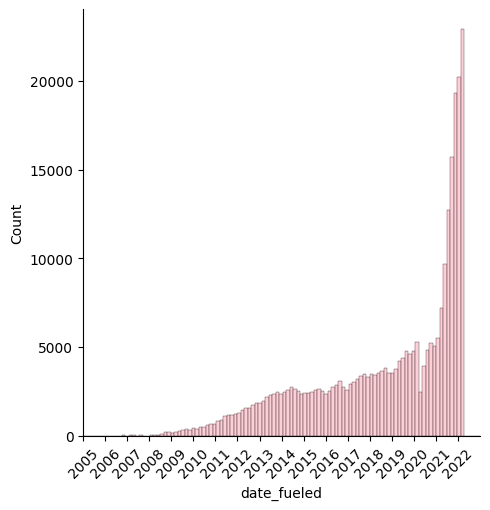
\includegraphics[width=0.6\textwidth]{images/fueled_dates_histo.png}
    \caption{Distribution of vehicle fueling dates. A significant drop in 2020 is attributed to COVID-19 quarantine regulations, followed by a recovery as restrictions were lifted.}
    \label{fig:fuel_dates}
\end{figure}
 
\end{enumerate}


\subsection{Numeric Fields}
The numeric fields \texttt{gallons}, \texttt{miles}, and \texttt{mpg} were cleaned as follows:
\begin{enumerate}
    \item The percentage of missing values was calculated for each field using \texttt{.isnull()}.
    \item Rows with two or more missing values from these fields were dropped to preserve data quality.
    \item Remaining missing values were imputed using the relationship $MPG = \frac{miles}{gallons}$.
    \item Commas in numeric strings were removed using \texttt{str.replace(',', '')} before conversion to type \texttt{float}.
\end{enumerate}

The distributions of the cleaned numeric fields are all right-skewed. The MPG distribution indicates most vehicles have lower fuel efficiency. The miles distribution is dominated by short trips (0--10,000 miles), and the gallons distribution shows most fuel purchases are small (0--2,500 gallons), with very few extreme values likely representing errors or large commercial vehicles.

\begin{figure}[htbp]
    \centering
    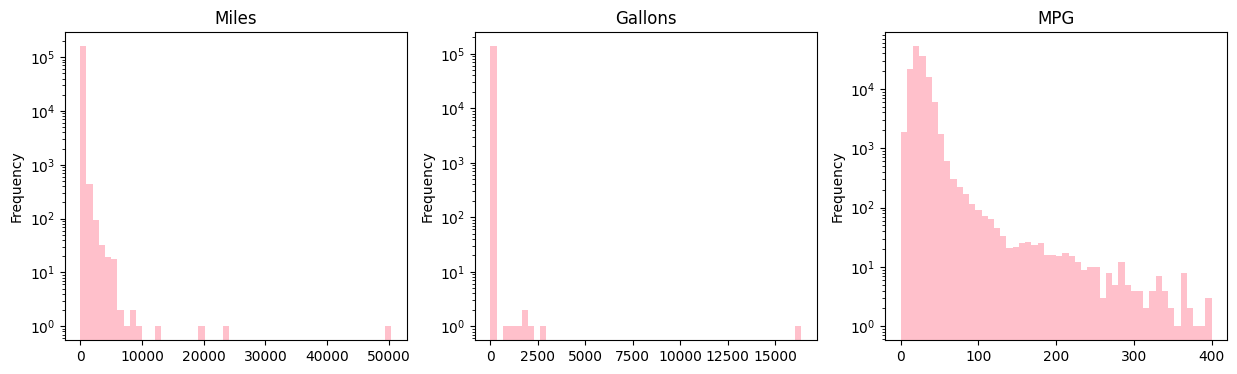
\includegraphics[width=0.6\textwidth]{images/numeric_distributions.png}
    \caption{Distribution of vehicle fueling dates. A significant drop in 2020 is attributed to COVID-19 quarantine regulations, followed by a recovery as restrictions were lifted.}
    \label{fig:fuel_dates}
\end{figure}


\section{Feature Engineering}
To enhance the dataset's utility, several new features were engineered:
\begin{itemize}
    \item \textbf{Currency Extraction:} Currency symbols (e.g., R, \$) were extracted from \texttt{total\_spent} and \texttt{cost\_per\_gallon} into a new \texttt{currency} column. The numeric parts were cleaned into floats.
    \item \textbf{User and Vehicle Information:} The \texttt{user\_url} field was parsed to extract a unique user ID, car make, model, and year.
    \item \textbf{Metric System Conversion:} Imperial units were converted to metric standards more common in South Africa:
    \begin{align*}
        \text{Litres Filled} &= \text{gallons} \times 3.785 \\
        \text{Kilometres Driven} &= \text{miles} \times 1.609 \\
        \text{Litres per 100km} &= (\text{litres} / \text{km\_driven}) \times 100
    \end{align*}
\end{itemize}
These new features standardize the data and enable more intuitive and region-specific analysis.

\section{Vehicle Exploration}

\subsection{Unique Users per Country}
Countries were proxied by their currency. \Cref{fig:users_per_country} shows that developed nations (e.g., USA, UK) have the largest user bases, while developing countries have the smallest, likely reflecting higher rates of personal vehicle ownership and app adoption in wealthier nations.

\begin{figure}[htbp]
    \centering
    \includegraphics[width=0.9\textwidth]{}
    \caption{Number of unique users per country, proxied by currency.}
    \label{fig:users_per_country}
\end{figure}

\subsection{App Popularity Over Time}
\Cref{fig:users_per_day} plots the number of unique users per day. The sharp increase in the 2010s and early 2020s correlates with the widespread adoption of smartphones and apps. The decline after 2022 is likely an artifact of data collection ending rather than a drop in actual popularity.

\begin{figure}[htbp]
    \centering
    \includegraphics[width=0.9\textwidth]{media/image5.png}
    \caption{Number of unique users per day, showing the app's growth over time.}
    \label{fig:users_per_day}
\end{figure}

\subsection{Vehicle Age Distribution by Country}
\Cref{fig:vehicle_age} shows the distribution of vehicle ages (based on fueling date) for the top 20 countries. Most vehicles globally are less than 20 years old, with a median age of approximately 10 years.

\begin{figure}[htbp]
    \centering
    \includegraphics[width=0.9\textwidth]{media/image4.png}
    \caption{Distribution of vehicle age per country.}
    \label{fig:vehicle_age}
\end{figure}

\subsection{Popular Vehicle Makes and Models}
The most popular car makes are Toyota, Ford, and BMW. The most popular models are the Civic, Jetta, and Land Cruiser (\Cref{fig:pop_models}).

\begin{figure}[htbp]
    \centering
    \begin{subfigure}[b]{0.45\textwidth}
        \centering
        \includegraphics[width=\textwidth]{media/image3.png}
        \caption{Popular car makes.}
    \end{subfigure}
    \hfill
    \begin{subfigure}[b]{0.45\textwidth}
        \centering
        \includegraphics[width=\textwidth]{media/image1.png}
        \caption{Popular car models.}
    \end{subfigure}
    \caption{Popularity of vehicle makes and models.}
    \label{fig:pop_models}
\end{figure}

\section{Fuel Usage and Outlier Removal}
For meaningful analysis, outliers were removed for the top five currencies (\$, £, CA\$, €, R).
\begin{enumerate}
    \item The 1st and 99th percentiles for key variables (\texttt{total\_spent}, \texttt{gallons}, etc.) were calculated for each currency.
    \item Rows outside these currency-specific thresholds were removed to eliminate extreme or implausible values.
    \item This process ensured subsequent analyses were based on realistic and comparable data, reducing skew and improving the reliability of statistical measures.
\end{enumerate}

\section{Conclusion}
This project successfully transformed a raw, inconsistent dataset into a clean, enriched resource for analysis. Through methodical data cleaning and insightful feature engineering, we were able to standardize the data and uncover significant trends. Key findings include the correlation between economic development and app usage, the relative youth of vehicle fleets in top user countries, and the market dominance of specific automotive brands. The methodologies developed here provide a robust framework for handling similar real-world datasets in the future.

\end{document}